\documentclass{beamer}
\usepackage{xcolor}
\usepackage[utf8]{inputenc}
\usepackage[english]{babel} 
\usepackage{listings}

\usepackage{parcolumns}


\usetheme{Madrid}
\usecolortheme{beaver}

\renewcommand{\emph}{\textcolor{red}}

%------------------------------------------------------------
%This block of code defines the information to appear in the
%Title page
\title[Resource Sharing] %optional
{Enabling resource sharing in dataflow circuits}

\author[Marmet] % (optional)
{Axel Marmet}

\institute[EPFL] % (optional)

\date[EPFL 2019] % (optional)

\logo{
\includegraphics[height=1cm]{EPFL_Logo_Digital_RGB_PROD-768x333.png}}

%End of title page configuration block
%------------------------------------------------------------



%------------------------------------------------------------
%The next block of commands puts the table of contents at the 
%beginning of each section and highlights the current section:

%\AtBeginSection[]
%{
%  \begin{frame}
%    \frametitle{Table of Contents}
%    \tableofcontents[currentsection]
%  \end{frame}
%}
%------------------------------------------------------------


\begin{document}

%The next statement creates the title page.
\frame{\titlepage}


%---------------------------------------------------------
%This block of code is for the table of contents after
%the title page
%\begin{frame}
%\frametitle{Table of Contents}
%\tableofcontents
%\end{frame}
%---------------------------------------------------------

\section{Basic Idea}
\begin{frame}[fragile]
\frametitle{Motivation}
\begin{columns}[T]
    \begin{column}{0.45\textwidth}
      \begin{itemize}
          \item New iteration every two clock cycles
          \item Each multiplier has an occupancy of $0.5$
          \item Using only one multiplier would not hurt performance but diminish size of circuit
      \end{itemize}
    \end{column}
    \begin{column}{0.1\textwidth}
    \end{column}
    \begin{column}{0.45\textwidth}
      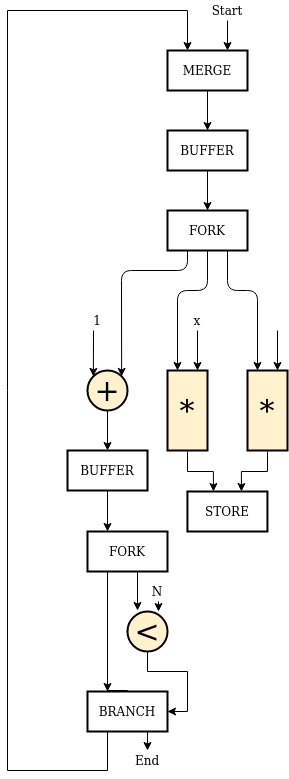
\includegraphics[scale=0.28]{base_case.png}
    \end{column}
  \end{columns}
\end{frame}

\begin{frame}[fragile]
\frametitle{Initial idea}
\begin{columns}[T]
    \begin{column}{0.45\textwidth}
    We add two new components to enable sharing \newline
    \begin{description}
        \item[Selector] Responsible for selecting inputs in a way that ensures fairness and will never deadlock
        \item[Distributor] Must send the resulting token to the correct outputs, is told where to send by the Selector through a FIFO
    \end{description}
    \end{column}
    \begin{column}{0.1\textwidth}
    \end{column}
    \begin{column}{0.45\textwidth}
      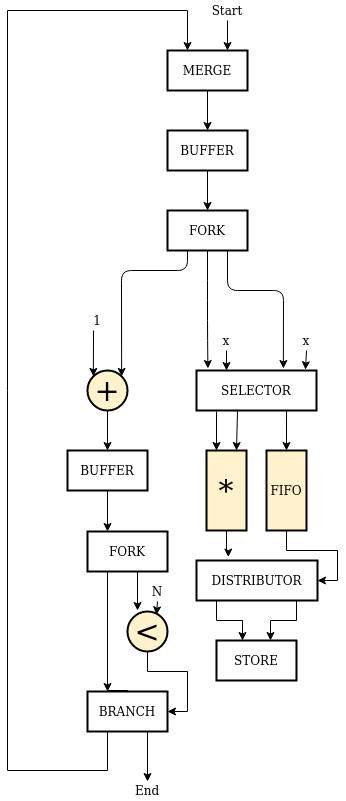
\includegraphics[scale=0.28]{shared_base_case.png}
    \end{column}
  \end{columns}
\end{frame}

\begin{frame}{Deadlock avoidance}
  How to schedule execution without causing deadlock ?
  \begin{columns}[T]
    \begin{column}{0.45\textwidth}
        How to schedule execution without causing deadlock ?
    \end{column}
    \begin{column}{0.1\textwidth}
    \end{column}
    \begin{column}{0.45\textwidth}
      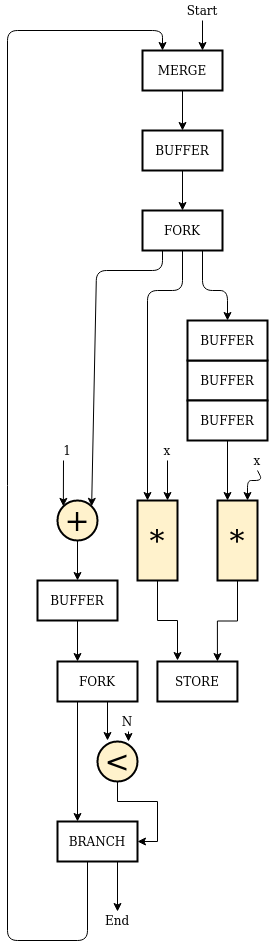
\includegraphics[scale=0.25]{blocking_unshared.png}
    \end{column}
  \end{columns}
\end{frame}

\section{Modification of the AST and Symbol table}
\begin{frame}{Modification to the AST}
Four new AST nodes :
\begin{itemize}
    \item MutVar
    \item Loop
    \item Branch
    \item Assign
\end{itemize}
\end{frame}

\section{}
\begin{frame}{Modification to the Symbol Table}
    Funsig that knows if tail rec or not
\end{frame}

\section{Parser}
\begin{frame}[fragile]{Parser}
     Simply need to modify function definitions and calls to signify if the function is tail rec or not. \\
     Proposed syntax :
     \begin{lstlisting}[basicstyle=\ttfamily]
     def a(arg1 : Type1)(acc : Type2) : Type3 = {
     
        ...
     
     }
     
     ...
     
     a(2)(3)
     \end{lstlisting}
\end{frame}

\section{TailRecPass}
\begin{frame}{TailRecChecker}
    Need to check the tail rec functions are indeed tail recs.\\
    Check that all exit statement is either a function call to itself with no other operation or a value.
\end{frame}

\begin{frame}{TailRecMaker}
    Assigns the arguments to new mutable variables.
    Transform the body of tail rec function using a loop/branch as in the example.
\end{frame}

\section{Inliner}
\begin{frame}{Inliner}
    Inline function body based on some heuristic (probably depth of the AST). 
\end{frame}

\begin{frame}[fragile]
\frametitle{ConstPropPass}
\begin{lstlisting}[basicstyle=\tiny\ttfamily]
    def fold(expr : Expr)(implicit consts : Map[Identifier, Literal[_]]) : Expr = 
        expr match {
        case Variable(name) => const.get(name) match {
            case Some(lit) => lit
            case None => expr
        }
        case Add(lhs, rhs) => (fold(lhs), fold(rhs)) match {
            case 
                (lit1:Literal[Int], 
                lit2: Literal[Int]) => 
                    literal(lit1.value + lit2.value)
            case (e1, e2) => Add(e1, e2)
        }
        case If(cond, thenn, elze) => fold(cond) match {
            case BooleanLiteral(b) => if (b) fold(thenn) else fold(elze)
            case folded => If(folded, fold(thenn), fold(elze))
        }
        // all binary and unary operations
        case Let(df, value, body) => 
            fold(value) match {
                case lit : Literal[_] => fold(body)(consts + (df.name -> i))
                case val => Let(df, val, fold(body));
            }
        case Match(scrut, cases) =>  /* if scrut is lit replace match by expr
                                        and in general fold all expressions on the rhs */
        ...
        case _ => expr
    }
\end{lstlisting}
\end{frame}

\begin{frame}[fragile]{OptiWasmPass}
    Replace obvious optimisations i.e.
    
    \begin{columns}
\begin{column}{0.45\textwidth}
   \begin{lstlisting}[keywords={}, basicstyle=\ttfamily]
    const 1 
    if 
        const 1
    else
        const 0
    end
    \end{lstlisting}
\end{column}
\begin{column}{0.1\textwidth}
   $\rightarrow$
\end{column}
\begin{column}{0.45\textwidth}
   \begin{lstlisting}[keywords={}, basicstyle=\ttfamily]
    const 1
    \end{lstlisting}
\end{column}
\end{columns}
    or 
    \begin{columns}
    \begin{column}{0.45\textwidth}
   \begin{lstlisting}[keywords={}, basicstyle=\ttfamily]
    set idx
    get idx
    \end{lstlisting}
\end{column}
\begin{column}{0.1\textwidth}
   $\rightarrow$
\end{column}
\begin{column}{0.45\textwidth}
   \begin{lstlisting}[keywords={}, basicstyle=\ttfamily]
    tee idx
    \end{lstlisting}
\end{column}
\end{columns}
\end{frame}

\end{document}